\documentclass[12pt,letterpaper]{article}
\usepackage[margin=1in]{geometry}
\usepackage{graphicx}
\usepackage{tabularx}
\usepackage{hyperref}
\usepackage{titlesec}
\usepackage{enumitem}
\usepackage{float}
\usepackage{booktabs}
\usepackage{tikz}
\usetikzlibrary{shapes.geometric, arrows.meta, positioning}

\hypersetup{
    colorlinks=true,
    linkcolor=blue,
    filecolor=magenta,      
    urlcolor=blue,
    pdftitle={Assignment 5: CI/CD Pipeline},
}

\setlength{\parindent}{0pt}
\setlength{\parskip}{0.8em}

\begin{document}

\begin{center}
    \Large\textbf{DevOps CS316 - Assignment \#5: CI/CD Pipeline with Git, GitHub Actions and Docker}
\end{center}

\vspace{0.5cm}

\begin{center}
    \begin{tabularx}{\textwidth}{@{}X X@{}}
        \textbf{Member 1:} Muhammad Hashir | Reg\# 2023429 & \textbf{Course Code:} CS316 \\
        \textbf{Member 2:} Zain ul Abdeen | Reg\# 2023773 & \textbf{Instructor:} Muhammad Sajid Ali \\
        \textbf{Date:} May 2026 & \textbf{Total Marks:} 100 \\
    \end{tabularx}
\end{center}

\vspace{1cm}

\section*{A. Project Introduction}
For this assignment, we successfully containerized a MERN stack application (Task Manager) and implemented an automated Continuous Integration and Continuous Deployment (CI/CD) pipeline. Using GitHub Actions workflows, the pipeline automates the builds, pushes tagged Docker images to the AWS Elastic Container Registry (ECR), and seamlessly deploys them to distinct AWS EC2 instances representing our Testing and Staging environments.

\section*{B. Challenges Faced}
During the implementation of the CI/CD pipeline and AWS cloud deployment, we encountered and resolved the following key challenges:

\begin{itemize}
    \item \textbf{Windows SSH Key Permissions:} 
    The \texttt{.pem} key threw a ``Bad permissions'' error on Windows when attempting to connect to the EC2 instances. We resolved this using PowerShell \texttt{icacls.exe} commands to strip inherited permissions and grant explicit read-only access to the current Windows user, fulfilling the strict SSH key security requirements.

    \item \textbf{AWS Authentication in GitHub Actions:} 
    The CI/CD pipeline needed secure access to push images to ECR. We solved this by creating a dedicated IAM User (\texttt{github-actions-deployer}) equipped with the \texttt{AmazonEC2ContainerRegistryPowerUser} policy, and securely storing the generated access keys in GitHub Secrets for the workflow to use.

    \item \textbf{Docker Compose Version Syntax:} 
    Automated deployment initially failed on the Ubuntu 24.04 EC2 instances because they defaulted to the modern Docker Compose V2 plugin. We successfully resolved this by updating the GitHub Actions workflow deployment script to use the new \texttt{docker compose} command (with a space) instead of the deprecated \texttt{docker-compose} format (with a hyphen).

    \item \textbf{React Environment Variables in Docker:} 
    The frontend application required configuration for the public backend API depending on whether it was deployed to Testing or Staging. Since React embeds environment variables at build time, we dynamically resolved this by passing \texttt{REACT\_APP\_API\_URL} as a build argument (\texttt{--build-arg}) inside our GitHub Actions workflow during the Docker build process.
\end{itemize}

\section*{C. Complete Flow Diagram}
The following architecture mapping and workflow table outline the comprehensive CI/CD workflow extending from the developer's initial push to the final staging deployment:

\begin{figure}[H]
    \centering
    \resizebox{\textwidth}{!}{
    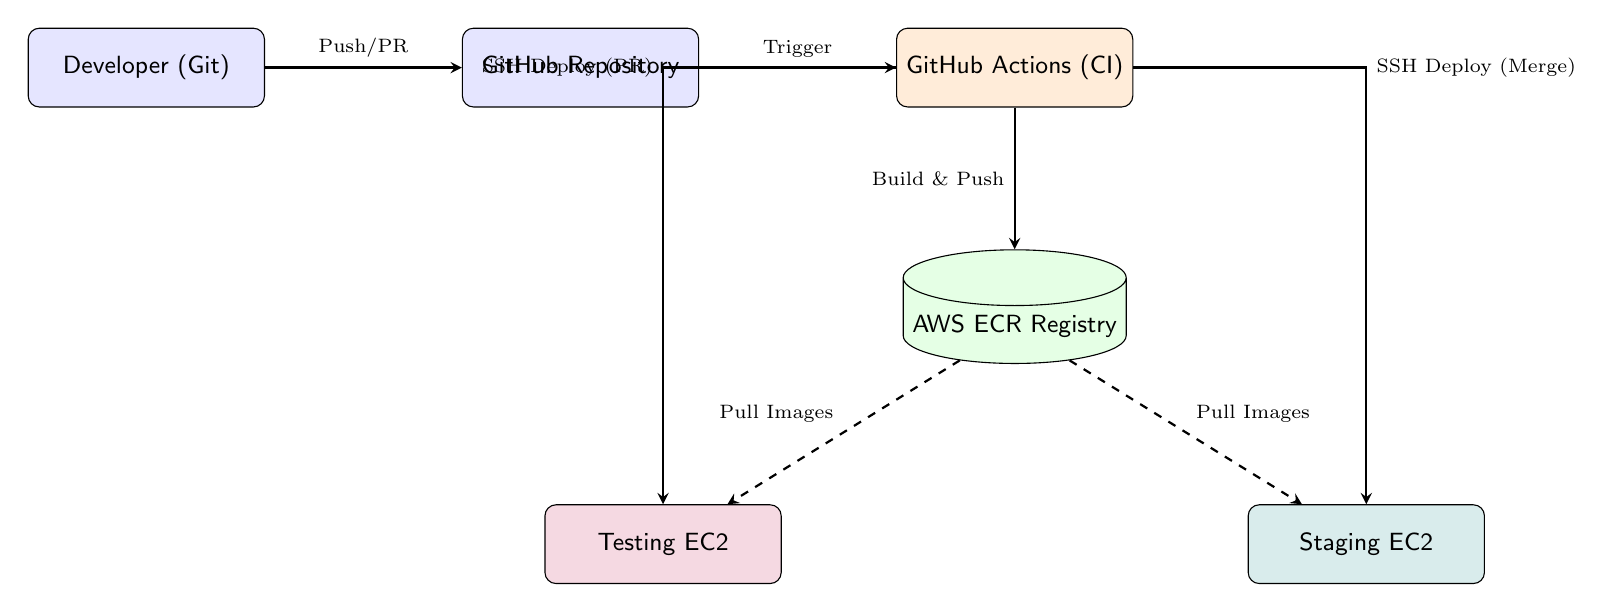
\begin{tikzpicture}[
        node distance=1.8cm and 2.5cm,
        process/.style={rectangle, rounded corners, minimum width=3cm, minimum height=1cm, text centered, draw=black, fill=blue!10, font=\small\sffamily},
        database/.style={cylinder, shape border rotate=90, aspect=0.25, minimum width=2.5cm, minimum height=1.2cm, text centered, draw=black, fill=green!10, font=\small\sffamily},
        arrow/.style={thick, ->, >=stealth}
    ]
        % Nodes
        \node (dev) [process] {Developer (Git)};
        \node (github) [process, right=of dev] {GitHub Repository};
        \node (actions) [process, right=of github, fill=orange!15] {GitHub Actions (CI)};
        \node (ecr) [database, below=of actions] {AWS ECR Registry};
        
        \node (testing) [process, below left=of ecr, fill=purple!15] {Testing EC2};
        \node (staging) [process, below right=of ecr, fill=teal!15] {Staging EC2};

        % Arrows
        \draw [arrow] (dev) -- node[anchor=south, font=\scriptsize] {Push/PR} (github);
        \draw [arrow] (github) -- node[anchor=south, font=\scriptsize] {Trigger} (actions);
        \draw [arrow] (actions) -- node[anchor=east, font=\scriptsize] {Build \& Push} (ecr);
        
        \draw [arrow] (actions) -| node[anchor=east, font=\scriptsize] {SSH Deploy (PR)} (testing);
        \draw [arrow] (actions) -| node[anchor=west, font=\scriptsize] {SSH Deploy (Merge)} (staging);
        
        \draw [arrow, dashed] (ecr) -- node[anchor=south east, font=\scriptsize] {Pull Images} (testing);
        \draw [arrow, dashed] (ecr) -- node[anchor=south west, font=\scriptsize] {Pull Images} (staging);
    \end{tikzpicture}
    }
    \caption{CI/CD Architecture and Automation Flow.}
\end{figure}

\vspace{0.3cm}
\begin{table}[H]
    \centering
    \renewcommand{\arraystretch}{1.5}
    \begin{tabularx}{\textwidth}{|>{\raggedright\arraybackslash\hsize=0.3\hsize}X|>{\raggedright\arraybackslash\hsize=0.7\hsize}X|}
        \hline
        \textbf{Phase} & \textbf{Workflow Actions \& Automation Steps} \\
        \hline
        \textbf{Developer Workflow} & 
        1. Developer creates a feature branch.\\ 
        & 2. Code changes committed and pushed to GitHub.\\ 
        & 3. A Pull Request (PR) to \texttt{main} is opened.\\
        \hline
        \textbf{Testing Workflow} & 
        1. Triggered automatically on PR creation/update.\\
        & 2. Source code tested and linted via GitHub Actions.\\
        & 3. Docker images (Frontend/Backend) built and tagged.\\
        & 4. Images pushed to AWS ECR.\\
        & 5. SSH action accesses the Testing EC2 server.\\
        & 6. Server pulls latest images from ECR and runs \texttt{docker compose up -d}.\\
        & 7. Automated success email sent to QA with testing IP link.\\
        \hline
        \textbf{Staging Workflow} & 
        1. Triggered automatically on PR merge into \texttt{main}.\\
        & 2. Codebase verified against \texttt{main}.\\
        & 3. Fresh Docker images built and pushed to AWS ECR.\\
        & 4. SSH action accesses the Staging EC2 server.\\
        & 5. Server pulls latest images and redeploys containers.\\
        & 6. Automated success email sent to Team with Staging IP link.\\
        \hline
    \end{tabularx}
\end{table}

\section*{D. Deployment Diagram Description}
The application deployment architecture utilizes separate Docker containers running concurrently on an AWS EC2 instance. The React frontend container serves the progressive user interface, while the Node.js backend container handles API integration and business logic. Both application containers securely communicate with a containerized MongoDB database instance over an isolated Docker network, ensuring encrypted data handling, portability, and efficient resource allocation.

\section*{E. Screenshots}

\subsection*{Task 1: Containerization and Local Setup}

Initially, the Task Manager component applications were containerized and verified to run successfully on a local developer machine using \texttt{docker-compose}.

\begin{figure}[H]
    \centering
    \includegraphics[width=0.75\textwidth]{"sc/1. vs code project tree"}
    \caption{Local Docker containers running via docker-compose.}
\end{figure}

\subsection*{Task 2: AWS Infrastructure}

To support our automated deployment, distinct EC2 environments were provisioned and linked to our Amazon ECR repositories utilizing secure IAM roles.

\begin{figure}[H]
    \centering
    \includegraphics[width=0.75\textwidth]{"sc/Running Instances in AWS"}
    \caption{AWS EC2 dashboard showing Dev, Testing, and Staging instances running.}
\end{figure}

\begin{figure}[H]
    \centering
    \includegraphics[width=0.75\textwidth]{"sc/ECR created repositories"}
    \caption{AWS ECR showing the taskmanager\_frontend and taskmanager\_backend repositories.}
\end{figure}

\begin{figure}[H]
    \centering
    \includegraphics[width=0.75\textwidth]{"sc/IAM role attached to dev enviormnet"}
    \caption{AWS IAM role showing the AmazonEC2ContainerRegistryReadOnly policy attached to the EC2 instances.}
\end{figure}

\begin{figure}[H]
    \centering
    \includegraphics[width=0.75\textwidth]{"sc/IAM role"}
    \caption{AWS IAM role details highlighting ECR permissions.}
\end{figure}

\begin{figure}[H]
    \centering
    \includegraphics[width=0.75\textwidth]{"sc/IAM User created"}
    \caption{Dedicated AWS IAM User created for GitHub Actions deployment capabilities.}
\end{figure}

\begin{figure}[H]
    \centering
    \includegraphics[width=0.75\textwidth]{"sc/security group details"}
    \caption{EC2 Security Group configurations allowing required inbound traffic.}
\end{figure}

\subsection*{Task 3: GitHub Actions CI/CD Workflows}

The complete pipeline requires extensive identity integration. After securing our GitHub repository with AWS credentials, we validated both the Testing workflow triggered by a PR and the Staging Workflow upon merging.

\begin{figure}[H]
    \centering
    \includegraphics[width=0.75\textwidth]{"sc/testing.yml in vscode"}
    \caption{VS Code environment showing the customized testing.yml GitHub Actions workflow.}
\end{figure}

\begin{figure}[H]
    \centering
    \includegraphics[width=0.75\textwidth]{"sc/Secrets in repo"}
    \caption{GitHub Actions Secrets page showing AWS and Email configuration.}
\end{figure}

\begin{figure}[H]
    \centering
    \includegraphics[width=0.75\textwidth]{"sc/ssh established"}
    \caption{Testing EC2 terminal showing the production docker-compose.yml configured with ECR URIs.}
\end{figure}

\textbf{Testing Environment Deployment Verification}

\begin{figure}[H]
    \centering
    \includegraphics[width=0.75\textwidth]{"sc/testing workflow success run on github"}
    \caption{GitHub Actions tab showing the Testing workflow passing (green checkmarks).}
\end{figure}

\begin{figure}[H]
    \centering
    
\includegraphics[width=0.75\textwidth]{"sc/testing successful email .png"}
    \caption{Automated QA success email showing the Testing server IP link.}
\end{figure}

\begin{figure}[H]
    \centering
    \includegraphics[width=0.75\textwidth]{"sc/live app on testing instance link"}
    \caption{Browser showing the application running live on the Testing EC2 instance.}
\end{figure}

\textbf{Staging Environment Post-Merge Deployment}

\begin{figure}[H]
    \centering
    \includegraphics[width=0.75\textwidth]{"sc/pull requestest successfull merge"}
    \caption{Pull request successfully approved and merged into the main branch.}
\end{figure}

\begin{figure}[H]
    \centering
    \includegraphics[width=0.75\textwidth]{"sc/staging workflow success on github"}
    \caption{GitHub Actions tab showing the Staging workflow passing after merging the PR.}
\end{figure}

\begin{figure}[H]
    \centering
    \includegraphics[width=0.75\textwidth]{"sc/docker compose on staging"}
    \caption{Staging EC2 terminal showing docker compose successfully pulling and deploying images.}
\end{figure}

\begin{figure}[H]
    \centering
    \includegraphics[width=0.75\textwidth]{"sc/staging successful deployed email"}
    \caption{Automated Team success email showing the Staging server IP link.}
\end{figure}

\begin{figure}[H]
    \centering
    \includegraphics[width=0.75\textwidth]{"sc/live app on staging instance"}
    \caption{Browser showing the application running live on the Staging EC2 instance.}
\end{figure}

\end{document}